In this Section we will focus on discrete-variable systems. Special attention will be payed to Noisy Intermediate-Scale Quantum (NISQ) computing, a concept standing for currently available technologies, where quantum circuits of about $50-100$ qubits are already being implemented and controlled despite the strong presence of noise~\cite{preskill2018quantum}.

While error-correcting codes cannot be built with such a low amount of qubits ---it is estimated that nearly a thousand \textit{physical qubits} are required in order to get a single \textit{logical qubit}~\cite{Fowler2012surface}--- special-purpose quantum devices can readily be built, exhibiting a genuinely quantum behaviour. Whether such techologies will be able to provide a game-changer quantum advantage in industry applications, or they are just a stepping stone towards fault-tolerant architectures is a matter of vivid debate between the community~\cite{supremacygoogle,nosupremacy,chemistrynono}. However, we remark that the sole feasibility of experimental preparation and control of quantum systems already constitute a game-changer paradigm in our scientific community. In turn, not only a plethora of new questions regarding scalability and overall implementation of such techologies arise~\cite{useful2discoverQC}, but also the demand for new theoretical tools, particularly to better analyze performance issues that we will later discuss~\cite{mcclean2018barren,cerezo2020cost,pesah2020absence,holmes2020barren,zhao2021analyzing,thanasilp2021subtleties,sharma2020trainability,patti2020entanglement,marrero2020entanglement,cerezo2020impact,arrasmith2020effect, npHardVQA}.

In the following we will concentrate on an specific topic that falls under the umbrella of NISQ computing, called Variational Quantum Algorithms.

\subsection{Variational Quantum algorithms}\label{ssec:1_nisq_vqa}
Recently, a superpisition of hype and hope has been put on the  %~\cite{preskill2018quantum, peruzzo2014variational, pesah2021absense,sharma2022reformulation,biamonte2017quantum
field of quantum machine learning~\cite{biamonte2017quantum, supremacygoogle, schuld2021isquantum, Aaronson2015, preskill2018quantum, peruzzo2014variational, pesah2021absense,sharma2022reformulation}, particularly when \textit{training} Parametrized Quantum Circuits (PQCs).

PQCs consists on a series of quantum gates, \textit{e.g.} CNOTs and rotations, where the real parameters of the latter are modified in order to \textit{optimize} the circuit. Here, and in analogy to the classical neural networks scenario~\cite{Goodfellow-et-al-2016}, we aim to minimize a given cost function (and thereby, these circuits are also known as \textit{quantum neural networks}). The overall training of PQCs is known as a Variational Quantum Algorithm (VQA), and consists on an hybdrid classical-quantum scheme. In turn, a quantum device is only used to estimate cost-function values, whereas a classical algortihm is in charge of controlling that quantum device by optimizing over accessible degrees of freedom, \textit{e.g.} rotation parameter values. Recently, many efforts have been carried out in order to analyze the performance, trainability and overall feasibility of VQAs~\cite{VQA_revmarco, VQA_revalba}.

Training a VQA means to solve an optimization problem encoded into a cost function of the form
\begin{equation}\label{eq:cost}
    C(\kvec,\thv)=\sum_i^M f_i\left(\tr{\Oi U(\kvec,\thv)\rho_i U^\dagger (\kvec,\thv)}\right)  \,.
\end{equation}
Here, $\{\rho_i\}$ are $n$-qubit states forming a \textit{training set} of cardinality $M$, and $U(\kvec,\thv)$ is our NISQ circuit parametrized by continuous parameters $\thv$ (\textit{e.g.}, rotation angles) and by discrete parameters $\kvec$ (\textit{e.g.}, gate placements). Moreover, $\Oi$ are observables and $f_i$ are functions that encode the optimization task at hand.

For example, when employing the Variational Quantum Eigensolver (VQE) algorithm~\cite{peruzzo2014variational} we have $f_i(x)=x$ and the cost function reduces to
\eq{vqe_cost}{C_{\text{VQE}}(\kvec,\thv)=\tr{\hat{H} U(\kvec,\thv)\rho U^\dagger (\kvec,\thv)},}where $\rho$ is the input state (and the only state in the training set) and $H$ is the Hamiltonian whose ground state we seek to prepare. Alternatively, in a classification problem where the training set is of the form $\{\rho_i,y_i\}$, with $y_i\in \{1,...,n\}$ being the true label, the choice $f_i(x)=(x-y_i)^2$ leads to the least square error cost~\cite{classiVQA, vqaclass1, vqaclass2,vqaclass4, cong2019quantum}.
In this regard, and as it happens in the reinforcement-learning scenario discussed in Sec.~\ref{sec:1_rl}, the possibility of encoding a given problem into a cost function is a matter of creativity.

\vspace{1cm}

Given the cost function, a NISQ circuit is employed to estimate each term in Eq.~\eqref{eq:cost}. Ussually, the available measurements consist on local projections over the eigenbasis of $\sigma^{i}_z$ for each qubit $i=1,...,n$. Here, in order to estimate the cost function, we decompose each operator appearing in the cost-function in terms of \textit{Pauli-strings}. Recall that Pauli-string operators form a basis in the space of $n$-dimensional hermitian operators and hence
\eq{decoH}{ \Oi = \sum_{k=1}^{4^n} c_k P_k,}
with $P_k = \bigotimes_{i=1}^n\mathbb{\sigma}_j$, where $\mathbb{\sigma}_j \in \llaves{\mathbb{I}, \sigma_x, \sigma_y, \sigma_z}$. Note that Pauli-string operators are orthogonal to each other, \textit{i.e.} $\tr{P_k P_{k'}} = 2^n \delta_{k k'}$ and thus $c_k = \tr{\Oi P_k}/2^n$.

Thus, the cost-function can be estimated by computing averages of some pre-determined observables, which are in turn a weighted sum of expected values of Pauli-strings. Moreover, we can estimate each expected value $\langle P_k\rangle$ by performing the corresponding single-qubit transformation beforehand and measuring $\sigma_z$\footnote{This can be understood as a change-of-basis.}. In this regard, if an $\epsilon$-accuracy is required in order to estimate this expected value, an order of $\sim \frac{1}{\epsilon^2}$ measurements needs to be done (this will have consequences when trying to resolve between very small values of the cost-function in Sec.~\ref{ssec:1_nisq_barrenplateaus}).

We also note that the Pauli-string procedure outlined above consists on an exponentially large sum of expected values. However, we are often interested in local hamiltonians, where many of these terms vanish (for example, TFIM and XXZ models considered in Ch.~\ref{chapter:VANS}). In this case, techniques such as randomized measurements (RMs) have recently been developed, in which the cost function can be computed more efficiently. While we do not consider such approaches in this thesis, we refer the interested reader to Ref.~\cite{elben2022randomized}, and we note that a combination between our methods (discussed in Chapter~\ref{chapter:VANS}) and classical shadows (a sub-class of RMs) is discussed in Sec.~\ref{ssec:vans_discu}.

\vspace{1cm}

Once the cost-function has been estimated, the power of classical optimization algorithms is leveraged to solve the optimization task
\begin{equation}\label{eq:optimization}
    \argmin{\kvec,\thv} C(\kvec,\thv)\,.
\end{equation}
\begin{figure}[t!]
    \centering
    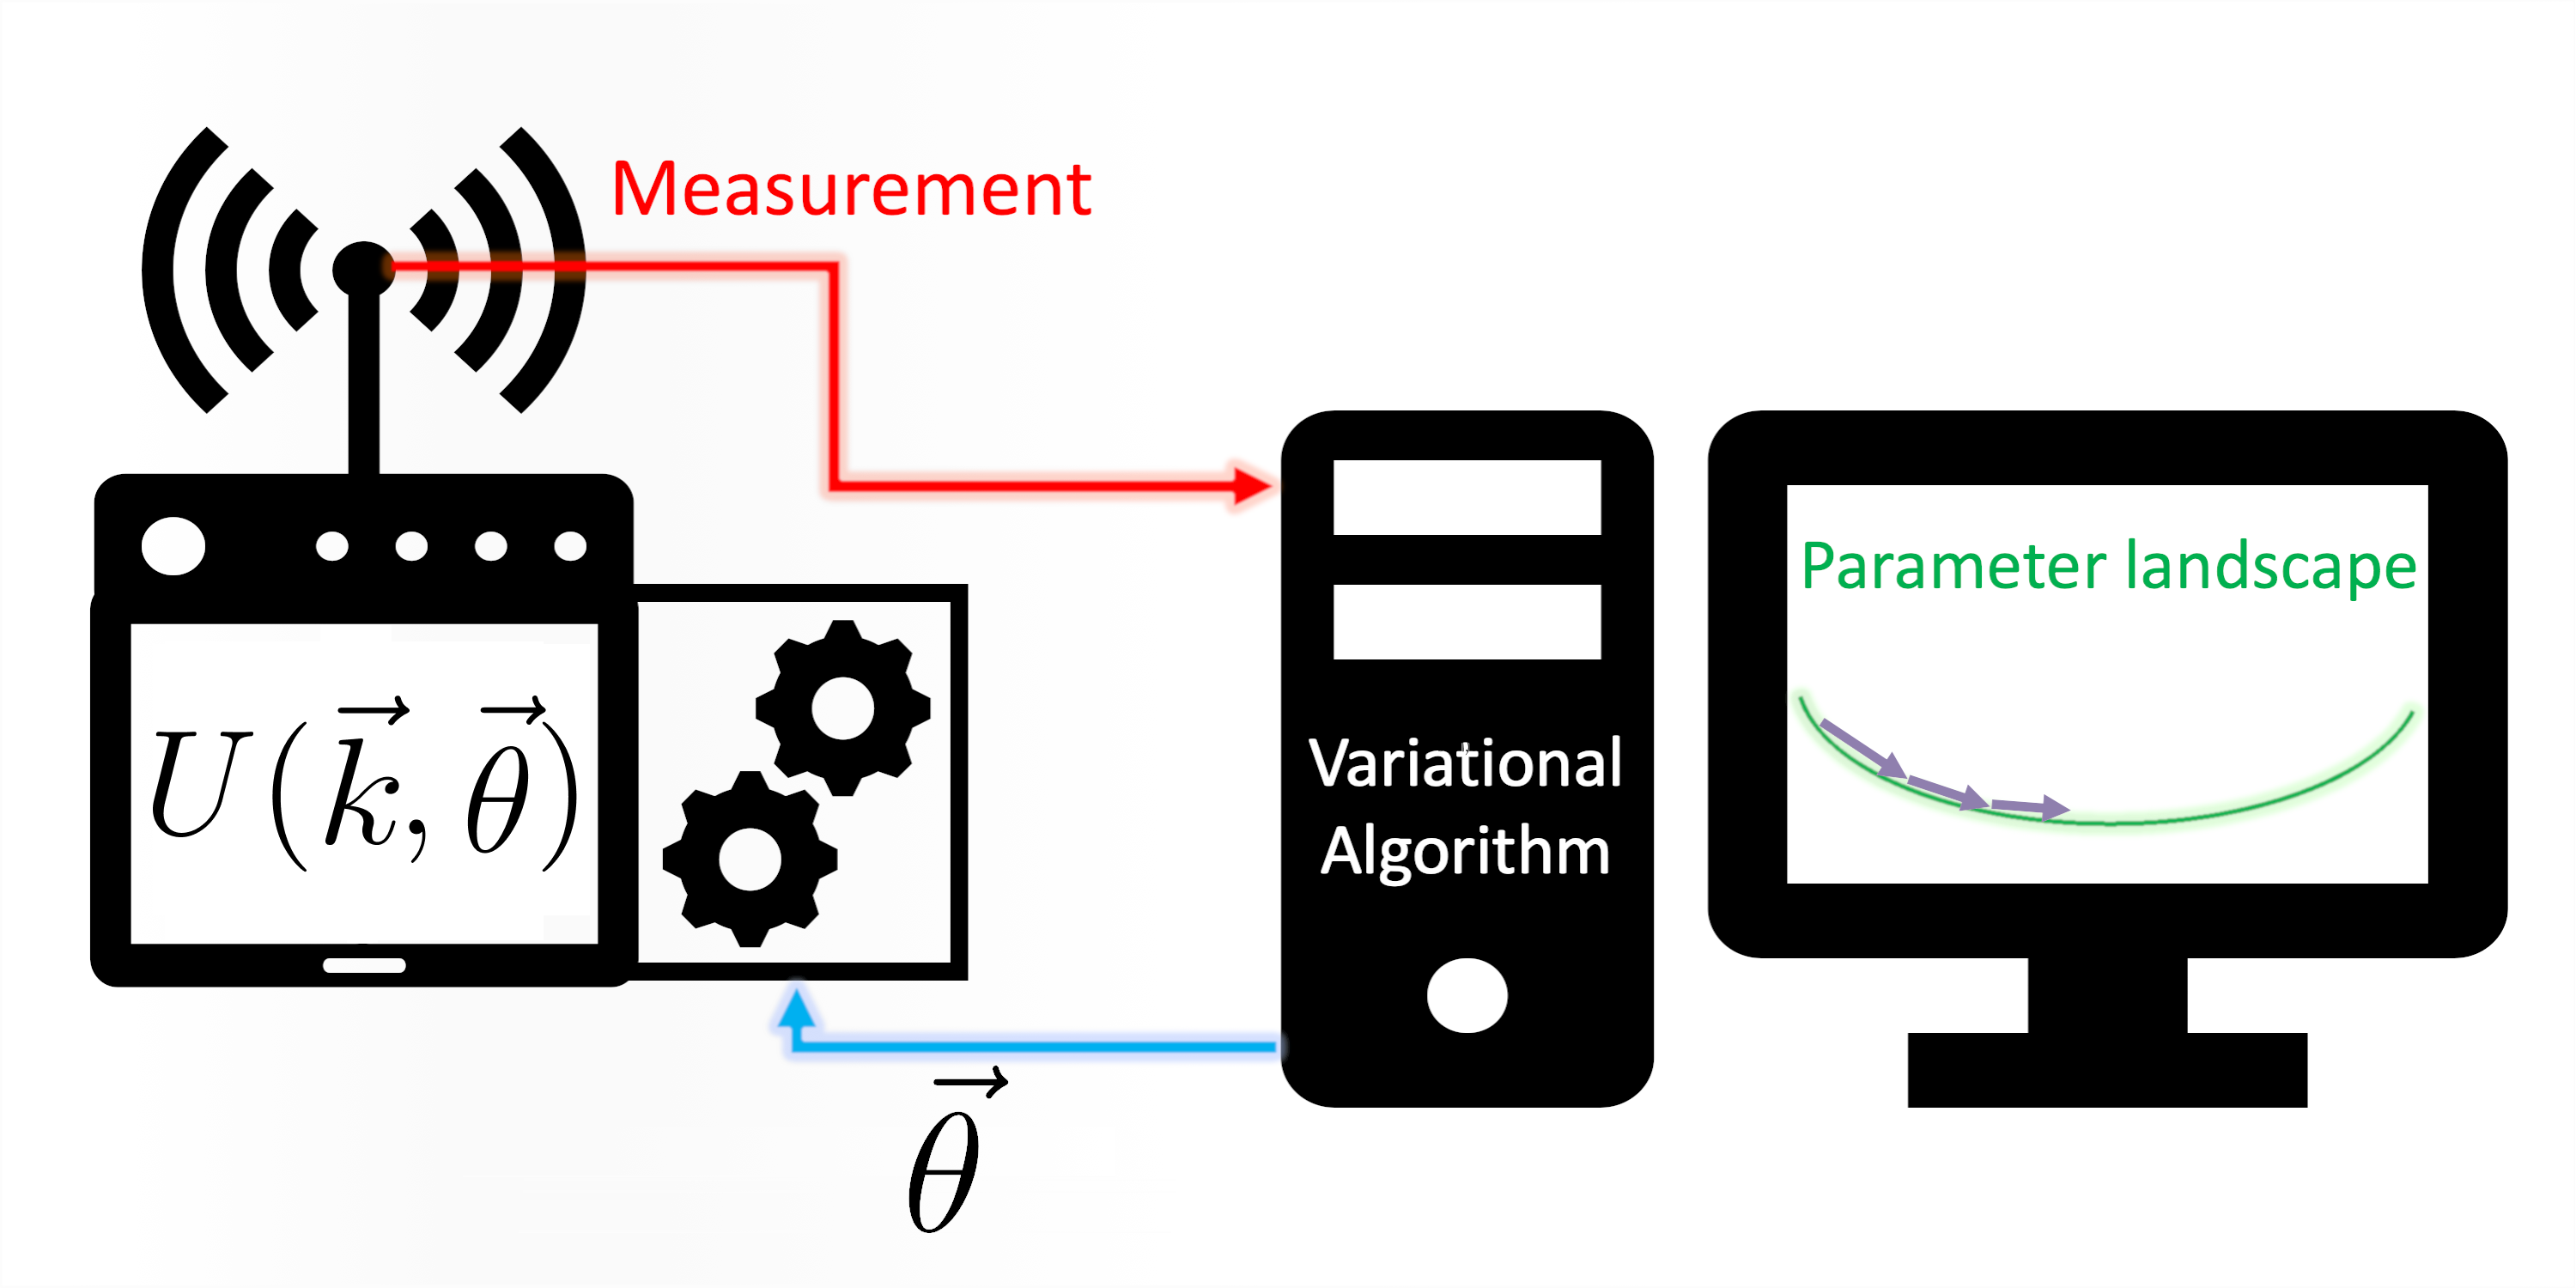
\includegraphics[width=1.\textwidth]{Figures/VANS/vqa_cycle.png}
    \caption{Figure adapted from Ref.~\cite{borrowed}: a generic VQA algortihm is sketched. Here, a quantum device is used to estimate a cost-function value, whereas the device itself is controlled by a classical optimization algorithm. This cycle is iterated until convergence.}
    \label{fig:VQAcycle}
\end{figure}
The estimation of a cost function via a quantum circuit and its modification (hopefully towards a cost-minimizing direction) by a classical optimization algorithm defines a cycle, which is repeated until convergence, as depicted in Fig.~\ref{fig:VQAcycle}. The success of such scheme hinges on several factors. As a matter of fact, the classical optimizer must be able to efficiently train the parameters, and in the past few years, there has been a tremendous effort in developing quantum-aware optimizers~\cite{verdon2018universal,kubler2020adaptive,arrasmith2020operator,stokes2020quantum,koczor2019quantum,nakanishi2020sequential,fontana2020optimizing}. In particular, severe trainability issues has been pointed out, which forbid the success of VQAs and as constitute the main barrer (along with hardware-noise) for making use of current NISQ devices in the VQA framework, and we will review some of them in Sec.~\ref{ssec:1_nisq_vans_bp}.

However, we note that even if such trainability issues could be overcomed, the performance of a VQA will intrinsically be linked to the specific quantum circuit used for the training. Here, the choice of an ansatz for $U(\kvec,\thv)$ plays a crucial role in determining the success of a VQA scheme; for instance, for a given Hamiltonian in the VQE algorithm, circuits that are close to the ground-state preparing one might lie outside the subspace $\mathcal{U}$ of the unitary group $U(n)$ which is generated by varying $\thv$ in $U(\kvec, \thv)$, with a fixed circuit layout given by $\kvec$~\cite{holmes2021connecting}.

In this respect, not every unitary transformation in $U(n)$ can straightforwardly be implemented, since the availability of quantum gates is often restricted; we generally need to deal with a \textit{gate-dictionary} $\mathcal{D}$, which in this thesis will be composed of one-qubit rotations and of CNOTs entangling any pair of qubits present in the circuit. We note that such an dictionary is universal~\cite{nielsen00}: any quantum gate can be implemented provided enough gates of the dictionary are used. Nevertheless, such a \textit{compilation} is a tricky one: noise accumulates with circuit's depth, and hence only a non-trivial set of unitaries can be reached. Moreover, we remark that the availability of fully-connected qubits is a slight simplification, and connectivity constraints should in principle be considered. In the latter case, entangling two qubits which are not straightforwardly connected represents an overhead in circuit's depth, and many efforts have been carried out recently in order to find novel strategies to tackle this issue~\cite{compilingDeepRLmaster}.

For these reasons, it is important to discuss different strategies ussually considered when constructing the quantum-circuit to be used in a VQA, also known as an \textit{ansatz}. %Here, we can readily distinguish between fixed-structure quantum circuits (where only the continuous paramters encoded in the rotations values are optimized), and variable-structure ones, in which both parameters \textit{and} strucure are optimized.


\subsection{The Ansatz}\label{ssec:1_nisq_vans_bp}
We refer to the \textit{ansatz} as the quantum-circuit structure, \textit{i.e.} the layout defining quantum-gates placements. While such a word stand for \textit{an educated guess or an additional assumption made to help solve a problem}~\cite{wikiansa}, let us remark that trainability and noise-related issues make it non-trivial to define what an \textit{educated guess} for a given problem is in the NISQ-era.

We will make a distinction between \textit{fixed}-structured ansatzes (\textit{i.e.} where $\kvec$ is fixed), and \textit{variable}-structure ones, in which also the structure of the circuit is optimized. In the latter case, the optimization is arguably more complex, since it consists on finding the right circuit structure on top of the continuous parameter optimization.

A key parameter that characterizes the ansatz is the number of gates present in the circuit. It is thus essential to construct ansatzes that maintain this number as low as possible to mitigate noise and trainability-related issues, but also that have enough expressibility to contain the problem solution (or at least an approximate version of it).

In the following we will first discuss some commonly-used fixed-structured ansatzes, and we will then turn to the variable-structure case.
% \subsubsection{Fixed-structure ansatzes}\label{sssec:blabla}

\vspace{1cm}

Let us now discuss on some commonly-used fixed-structure ansatzes. We first consider a \textit{separable} ansatz as depicted in Fig.~\ref{fig:FANSATZ}. Here, the structure is so trivial that no entanglement is generated by the circuit, since only local operations are performed on each qubit. Assuming that the initial state is separable ---we often consider it to be $\ket{0}^{\otimes n}$---, only a very small fraction of the Hilbert space can be reached under this circuit's choice~\cite{separableAnna}, and the overall performance is expected to be poor since the presence of entanglement is generally required. Also, note that the separable case can efficiently be simulated in a classical computer, and thus we do would not expect them to provide any quantum advantage.

\begin{figure}[t!]
    \centering
    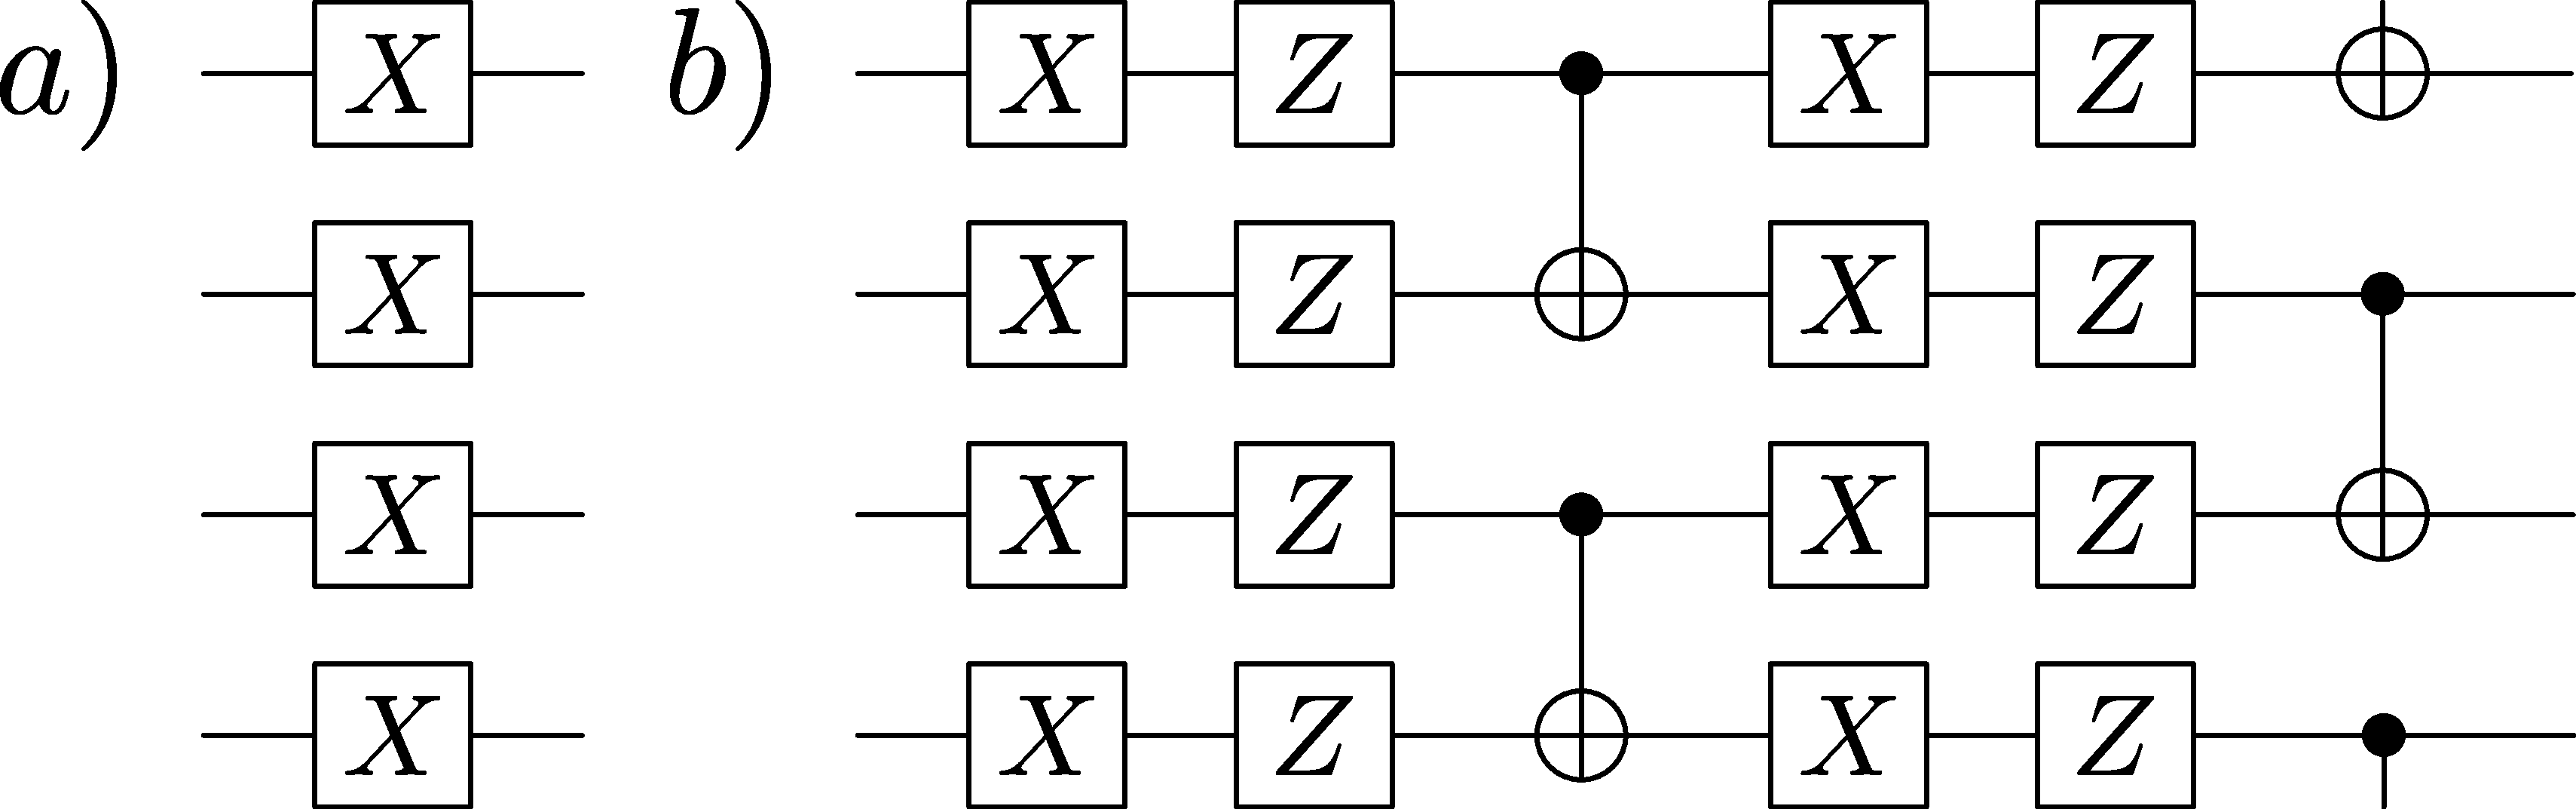
\includegraphics[width=1.\textwidth]{Figures/VANS/Fig2.pdf}
    \caption{We show examples of commonly-used quantum circuits. In \textit{(a)} we depict a separable product ansatz which generates no entanglement between the qubits. On the other hand, \textit{(b)} shows two layers of a shallow alternating Hardware Efficient Ansatz where neighboring  qubits are initially entangled.  Here $Z$ ($X$) indicates a parametrized rotation about the $z$ ($x$) axis (the angles $\bm{\theta}$ are not explicitely shown, but such are the degree of freedom to optimize over).}
    \label{fig:FANSATZ}
\end{figure}

This issue can be addressed with the layered Hardware Efficient Ansatz\cite{kandala2017hardware}, which we refer as HEA. Here, the gates are arranged in a brick-like fashion and act on alternating pairs of qubits, as depicted in Fig.~\ref{fig:FANSATZ}. We define a $L$-HEA as a circuit in which $L$ layers are stacked next to each other: a single layer consists on $n-1$ two-qubit gates (in the figure, rotations around $x$ and $z$ axis, followed by a CNOT) that correlate two neighbour qubits in the circuit. We here will consider the qubits as a cyclic chain, where the bottom one is also conected to the upper one, although this definition can be adapted to specific qubit-connection constraints of the quantum computer at hand. As $L$ increases, it can be expected that HEA becomes more expressible. as opposed to the separable circuit, whose expressibility is very poor.

In turn, HEA turns out to be \textit{too} expressible~\cite{holmes2021connecting}, in the sense that any unitary can be mimicked using enough HEA-layers, and this can lead to trainability issues. For a sufficiently-expressible PQC, the landscape of possible unitaries $\mathcal{U}$ that can be reached by varying its parameters turns to be hard to navigate, in the sense that the cost-function landscape becomes very flat, a phenomenon known as a \textit{barren plateau}. The latter fact constitute a big challenge for an optimization proccedure that needs to navigate such landscape and reach the lowest cost-function value, as discussed in Sec.~\ref{ssec:1_nisq_barrenplateaus}.

One of the main advantages of HEA is that it employs gates native to the specific device used, hence avoiding an unnecessary overhead in the number of gates present in the circuit, arising from compiling non-native unitaries into native gates (for instance, the building-blocks in the figure could be replaced with gates coming from another dictionary). This type of ansatz is \textit{problem-agnostic}, in the sense that it is expressible enough so that it can be generically employed for any task; in Chapter~\ref{chapter:VANS} we will often use this ansatz for benchmarking purposes.

On the other hand, a hint on the solution for the target problem to be solved by a quantum computer can, in principle, be helpful when building the ansatz. This claim should certainly holds in the ideal (\textit{e.g.} noise-less) scenario, and in VQAs, this is reflected by the so-called \textit{problem-inspired} ansatzes. Here the goal is to encode information of the problem into the ansatz's structure so the optimal solution of Eq.~\eqref{eq:optimization} exists within the parameter space without requiring high expressibility.

An example of such fixed-structure ansatzes is the Quantum Alternating Operator Ansatz (QAOA) for optimization problems, which is aimed to adiabatically prepare the ground-state of a \textit{problem}-hamiltonian, and thus alternates between a \textit{mixing} unitary and a \textit{problem} one. We will not discuss thse ansatzes here, and the interested reader can find more details in Refs.~\cite{farhi2014quantum,hadfield2019quantum}.

On a different note, considerable effort has been made in order to construct physically-inspired ansatzes in the field of quantum chemistry, and the Unitary Coupled Cluster (UCC) Ansatz~\cite{cao2019quantum,bartlett2007coupled} is an example of them. We will discuss the quantum-chemistry problem in greater detail in Sec.~\ref{ssec:molecular_ham_vans}. Essentially, we here seek to prepare the ground state of a molecular Hamiltonian, which (under the Born-Oppenheimer approximation) translates to solve a many-body fermionic system, known as the \textit{electronic-structure problem}.
While much insight from the classical methods that tackle this problem can be brought to the NISQ scenario, some issues raise up. Namely, we need to map the [UCC] ansatz from fermions to qubits, as well as the molecular Hamiltonian, since we are here targeting applications on digital quantum computers. Such mapping can be done by the Jordan-Wigner transform (or alternatively Bravi-Kitaev). Unfortunately, this ussually comes with an overhead in the number of quantum gates required to build the specific circuit (and also a large number of Pauli observables to represent the molecular Hamiltonian). This fact constitutes a big challenge for NISQ applications, since deep circuits are severely affected by noise.

We might think of quantum chemistry as a subset of problems that quantum computing can potentially addess. Generally, for a given physical problem, a family of quantum-circuit structures reflecting certain symmetries of potential solutions could in principle be constructed. However, quantum-hardware noise makes it highly no trivial to directly translate such physical intuition into the structure of the quantum circuit. %, since the afforementioned challenges related to noise generally arise.
\vspace{1cm}

Under the presence of limited resources, each component of the VQA that could in principle be optimized over, should be optimized over. This constitutes the spirit behind several efforts~\cite{grimsley2019adaptive,tang2019qubit,zhang2021mutual, rattew2019domain,chivilikhin2020mog, cincio2021machine, cincio2018learning,du2020quantum,zhang2020differentiable} to adapt the circuit layout to the specific scenario at hand (\textit{e.g.} a noise model, or the restricted availability of quantum hardware). In the following we will review some of such efforts, which are known as \textit{variable-structure ansatzes}. We remark that this is not the end of the story regarding optimization of VQA's components. As a matter of fact, we could also optimize the way cost-function estimates are obtained~\cite{algorithmiq1,algorithmiq2}, though we will only focus to optimizing circuit's structure.

The overall strategy of variable-structure ansatzes consists of iteratively changing the quantum circuit by placing (or removing) gates that empirically lower the cost-function value after the continuous-parameter optimization. The first proposal for variable ansatzes for quantum chemistry was introduced in~\cite{grimsley2019adaptive} under the name of ADAPT-VQE. Here, the authors follow a circuit structure similar to that used in the UCC ansatz introduced above, and propose to iteratively grow the circuit by appending gates that implement fermionic operators chosen from a pool of single and double excitation operators. At each iteration, one decides which operator in the pool is to be appended, which can lead to a considerable overhead if the number of operators in the pool is large. Similarly to the UCC case, the mapping from fermions to qubits can lead to prohibitively deep circuits. This issue can be overcomed using the qubit-ADAPT-VQE~\cite{tang2019qubit} algorithm, where the pool of operators is modified in such a way that only easily implementable gates are considered. However, the size of the pool still grows with the number of qubits. We refer the reader to~\cite{claudino2020benchmarking} for a detailed comparison between ADAPT-VQE and UCC ansatzes.

A different approach to variable-structure ansatzes that has gained considerable attention are machine-learning-aided evolutionary algorithms (EA) that upgrade individuals (quantum circuits) from a population. Noticeably, the presence of quantum correlations makes it so that it is not straightforward to combine features between circuits during the evolution, as simply merging two promising circuits does not necessarily lead to low cost-function values. Thus, only random mutations have been considered so far. An example of this method is found in the
Evolutionary VQE (EVQE)~\cite{rattew2019domain}, where one explores the Hilbert space \textit{smoothly} by growing the circuit with identity-initialized blocks of gates and randomly removing sequences of gates. Another example of an evolutionary algorithm is the Multi-objective Genetic VQE (MoG-VQE)~\cite{chivilikhin2020mog}, where one uses building blocks that are randomly placed along the circuit, and simultaneously optimizes both the energy and number of entangling gates. Evolutionary algorithms constitute a promising approach to ansatzes design, they nevertheless come at the cost of high quantum-computational resources to evolve populations of quantum circuits.

In addition, in Refs.~\cite{du2020quantum,zhang2020differentiable,pirhooshyaran2021quantum,du2020quantum} tools from auto-machine were employed in order to learn how to build ansatzes. The overall idea behind these methods is that of employing neural network (supernet) that suggests the quantum circuit structure; supernet-training can be done using policy-gradient methods, a variant of the reinforcement-learning algorithms that we consider in Sec.~\ref{sec:1_rl}. While the idea of artificial-intelligence improving (quantum) neural-network architectures is exciting, it is extremely resource-consuming: recall that the amount of data required to train a neural network is very often prohibitively high. Similarly to the EA case, the high amount of resources consumed by this method is a challenge that needs to be addressed.

Finally, in Refs.~\cite{cincio2018learning,cincio2021machine} a methodology, formalized by the VAns algorithm~\cite{bilkis2021semi} --- \textit{i.e.} our main contribution to the field, and explained and showcased in great detail in Chapter~\ref{chapter:VANS} --- was used to obtain a short-depth version of a given unitary under specific quantum hardware constraints (such as connectivity, noise-model as represented by quantum channels or available gates). %Explaining and showcasing our algorithm will be the matter of Chapter~\ref{chapter:VANS}.

Having reviewed some commonly-used quantum circuit structures, we will now turn to discuss the continuous optimization.


\subsection{The optimization procedure}\label{ssec:optimizer}
With a quantum circuit parametrized by $U(\kvec,\thv)$, VQAs employ a classical optimization algorithm in order to minimize the cost-function in Eq.~\eqref{eq:cost}. Here, we will focus on derivative-based methods, which at each cycle $\ell$ of the algorithm, the gradient $\nabla _{\thv} C(\kvec,\thv)$ is computed, and a cost-minimizing direction is followed. Ussually, the initial parameters $\thv^{\ell}$ are randomly chosen (this random initialization should be understood according to the Haar measure, as we discuss in the next Section). In the following we will first discuss about optimization algorithms, and then on how such gradients can be computed.

The most straightforward approach in gradient-based optimization is that of following the gradient; as such we are guaranteed to attain (at least) a local minima. Thus, in Gradient Descent algorithm, the continuous parameters are updated according to
\begin{equation}\label{eq:GD}
\thv^{(\ell + 1)} = \thv^{(\ell)} - \alpha \nabla _{\thv}(\kvec,\thv)|_{\thv = \thv^{(\ell)}},
\end{equation}
where $\alpha$ is the \textit{learning-rate}, accounting for the update-step size, and this is guaranteed to reach, at least, a local-minima.

In optimization problems where the dataset is too large, computing the gradients can be prohibitively expensive (for instance, if the entire dataset does not fit in the memory). In this case, the training set is splitted into chunks, and an stochasticity arises when estimating gradient; such is the case of Stochastic Gradient Descent (SGD), where the gradient is estimated out of $b$-dimensional data subsets known as \textit{batches}. At each cycle, the data is randomly splitted and the update rule of Eq.~\ref{eq:GD} is sequentially applied using the gradient $\nabla _{\thv} C(\kvec,\thv)$ computed using each batch (note that this injects stochasticity); an \textit{epoch} is consequently defined as an entire pass of the original training set. We note that this stochasticity, which might in principle appear undesired, it can actually be helpful since taking random directions often help in escaping local minima.

While a large learning-rate value in Eq.~\ref{eq:GD} can potentially forbid the optimizer to reach the actual minima (since the update becomes simply \textit{too large}), we note that small learning-rate values will potentially dampen the convergence rate. More elaborate optimization algorithms can be considered, which adapt the magnitude of the learning-rate according to the gradient landscape at hand. Among them, a very popular optimizer is the Adaptive Moment Estimation (Adam) algorithm~\cite{kingma2015adam}, which sequentially adapts the learning rate for each parameter, by specifically tailoring it out from moving averages of first and second moments for each gradient component. In practice, this allows to reach a better optimization performance, although we shall ultimately adapt the optimization algorithm to the specific problem at hand. In the context of VQA, many issues need to be addressed, such as shot-noise, sampling-complexity and optimal choice of learning-rate values to take into account the quantum nature of the optimization landscape; in this regard there has been a tremendous effort in developing quantum-aware optimizers~\cite{verdon2018universal,kubler2020adaptive,arrasmith2020operator,stokes2020quantum,koczor2019quantum,nakanishi2020sequential,fontana2020optimizing,gu2021adaptive}.

With a basic understanding on how optimization algorithms proceed, let us now discuss how the essential ingredient in the update-rule can be obtained under the VQA framework. For this, we distinguish between two approaches: \textit{(i)} classical simulation of quantum circuits, and \textit{(ii)} experimental implementations on quantum hardware.

\subsubsection{Classical simulation of quantum circuits $\&$ Automatic differentiation}
If no particular symmetries are imposed, we are able to simulate quantum systems classically for up to $\sim 30$ qubits\footnote{On the contrary, many systems can be approximated efficiently by using clever ansatzes; this lies at the heart of Tensor Network (TN) methods such as Matrix Product States (MPS), Density Matrix Renormalization Group (DMRG) or Multiscale Entanglement Renormalization Ansatz (MERA). There is currently much excitement about TNs: while the space of all possible quantum states is large, only a portion of it is \textit{physically relevant} and it is believed that such portion can be simulated efficiently using TNs~\cite{Biamonte2017tensornetworks,orusTN}.}.
%
State-of-the-art techniques used to classically compute VQA-cost-function gradients rely on automatic differentiation (AD), in which cost-function derivatives are obtained by tracking each intermmediate-operation derivative, and following the chain-rule~\cite{broughton2020tensorflow,Luo2020yaojlextensible}. This is done by decomposing a generic program in terms of elementary operations whose derivatives can be computed, and is the spirit behind the paradigm of \textit{differentiable programming}~\cite{Rackauckas2020GeneralizedPL,Liao2019differentaible,dpcontrolsto}.

We remark that AD differs from numerical differentiation (such as finite differences) since it is an exact method. Similarly to symbolic differentiation, each operation involved in the computation provides a rule for its derivative with respect to the corresponding input. However, the output of AD is a numerical value of the derivative, and not a mathematical expression for it.

In turn, AD is carried out by constructing a \textit{computational graph}, where nodes are associated to the elementary operations present in the computation (and whose derivatives are known), and where the dependence on the parameters is explicited. In order to compute the function derivative, the graph is transversed either forward or backwards; the latter case is known as \textit{backpropagation}\footnote{The optimal way to transverse the computational graph generally depends on the setting at hand. For high-dimensional inputs (as customary when working with neural networks), backpropagation is prefered at the cost of an increase in memory usage.}. Thanks to efficient matrix multiplication sub-routines and special-purpose hardware such as GPUs and TPUs, this can be done consideraly fast, and in turn AD stands as one of the main ideas behind the advent of Artificial Intelligence.

\begin{figure}[t!]
    \centering
    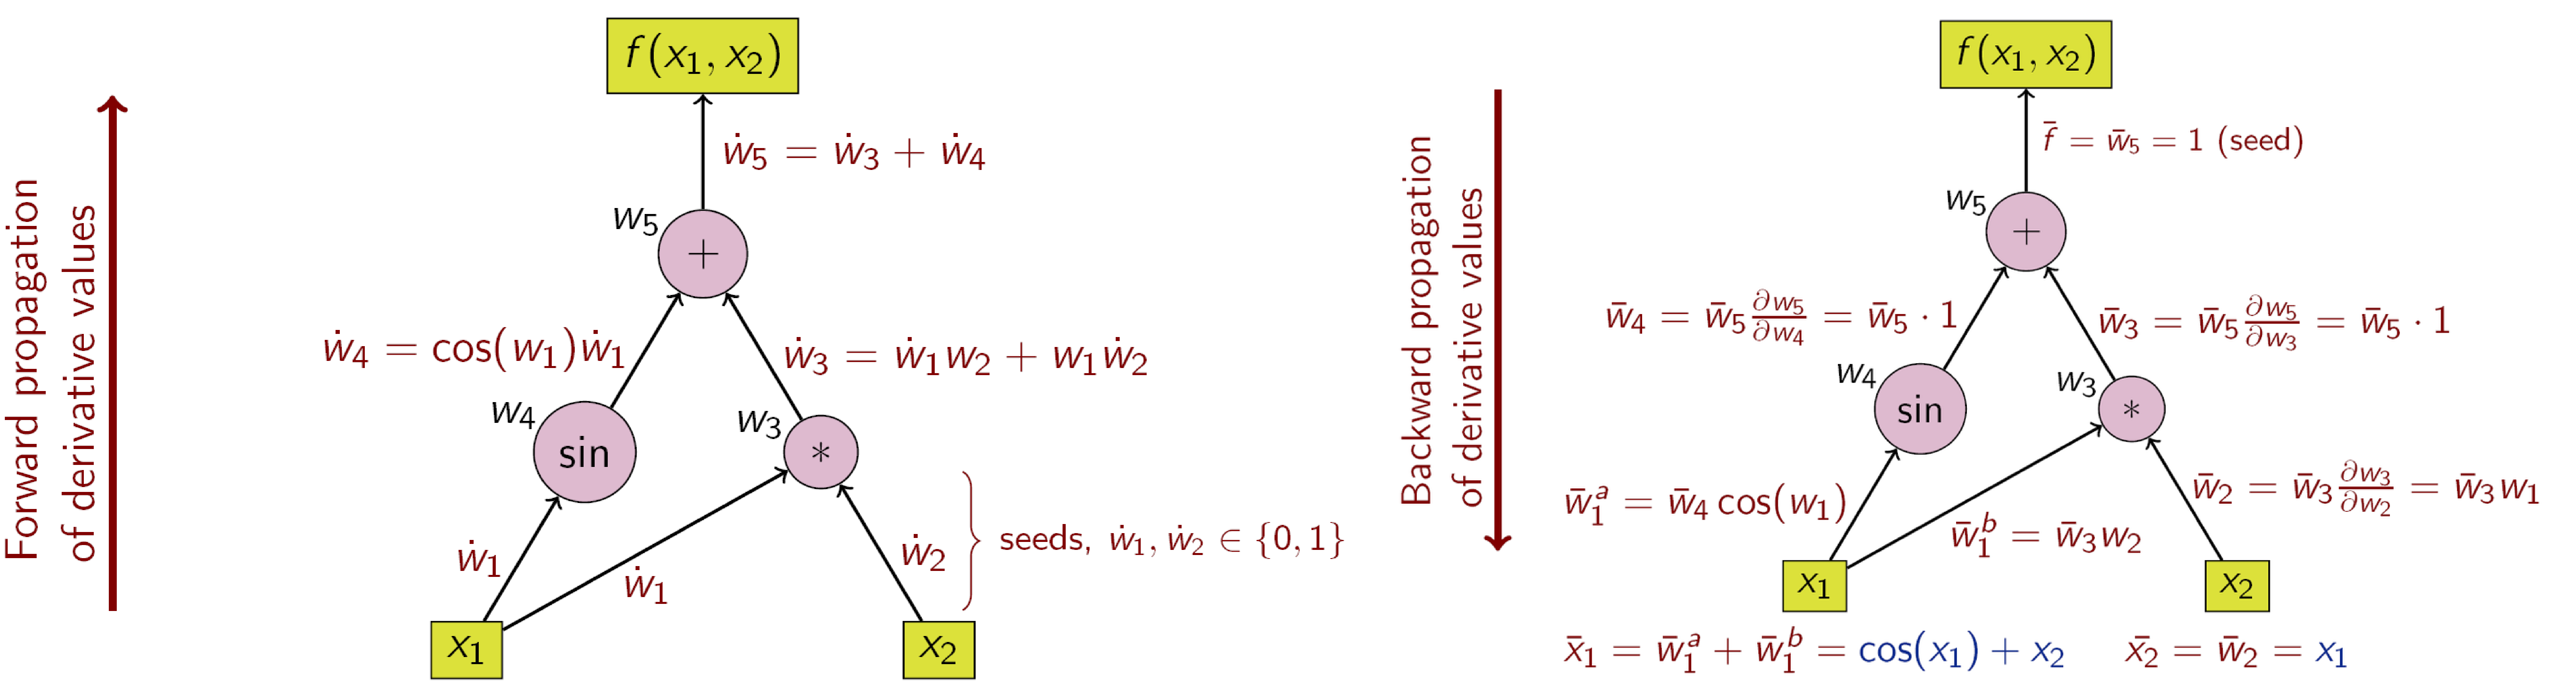
\includegraphics[width=1.\textwidth]{Figures/ad.pdf}
    \caption{We show how the computational graph is travelled forward and backwards in each of the possible modes of AD, for the example of an scalar function $f(x_1,x_2) = x_1 x_2 + \sin(x_1)$}
    \label{fig:ad}
\end{figure}

Let us consider an example\footnote{Taken from Ref.~\cite{wikiAD}} of an algorithm taking as input a real-value $x$, and outputing $y = f(g(h(x))$ where $f,g$ and $h$ are elementary functions whose derivatives are well-known and can be recorded when building the computational graph. We aim to compute $\partial_x y$, and to this end we define $w_0 = x$, $w_1 = h(w_0)$, $w_2 = g(w_1)$ and $w_3 = f(w_2) = y$. Now, the chain rule implies that
\equ{\frac{\partial y}{\partial x} = \frac{\partial y}{\partial w2} \frac{\partial w2}{\partial w1}  \frac{\partial w1}{\partial x}.} Thus, the computational graph is built by recording each of the elementary functions that need to be computed \textit{and} each of the elementary functions derivatives, which are known in advance. Then, forward-AD transverses the chain-rule from inside to outside, by first computing $\frac{\partial w_1}{\partial x}$, then $\frac{\partial w_2}{\partial w_1}$ and finally $\frac{\partial y}{\partial w_2}$.
On the contrary, backwards-AD transverses the chain-rule from outside to inside, by first computing $\frac{\partial y}{\partial w_2}$, then $\frac{w_2}{w_1}$ and finally $\frac{\partial w_1}{\partial x}$. As a concrete example, we can consider the function
\begin{align}
y &= f(x_1, x_2) \\
&= x_1 x_2 + \sin(x_1) \\ 
&= w_1 w_2 + \sin(w_1) \\
&= w_3 + w_4 \\
&= w_5,
\end{align}
where at each elementary operation we define a new variable $w_i$, which represents a node in the computational-graph. In the table we show the operations needed to compute the function, forward-AD, and backward-AD (this is also schematised in Fig.~\ref{fig:ad}).
\begin{center}
\begin{tabular}{| c |c |c |}
\hline
Function computation  &  Forward-AD&  Backward-AD\\
\hline
  $w_1 = x_1$&  $\dot{w}_1 = 1$ (\texttt{seed})&  $\bar{w}_5 = 1$ \texttt{seed}\\
  \hline
  $w_2 = x_2 $&  $\dot{w}_1 = 0$ (\texttt{seed})&  $\bar{w}_4 = \bar{w}_5 \cdot 1$\\
  \hline
  $w_3 = w_1\cdot w_2$& $\dot{w}_3 = \dot{w}_1\cdot w_2+ w_1 \cdot \dot{w}_2$ &  $\bar{w}_3 = \bar{w}_5 \cdot 1$\\
  \hline
  $w_4 = \sin(w_1)$& $\dot{w}_4 = \cos(w_1)\cdot \dot{w}_1$  &  $\bar{w}_2 = \bar{w}_3 \cdot w_1$\\
  \hline
  $w_5 = w_3 + w_4$& $\dot{w}_5 = \dot{w}_3 + \dot{w}_4$ &  $\bar{w}_1 = \bar{w}_3 \cdot w_2 + \bar{w}_4 \cos(w_1)$\\
  \hline
\end{tabular}
\end{center}
Here, we used the notation of $\bar{w}_i=\frac{\partial y}{\partial w_i}$ for the backward-AD, and note that the \textit{seed value} in this example is trivial for such case (since it stands for possible multidimensional outputs, \textit{e.g.} cases where $y \in \mathbb{R}^n$). On the contrary, since the example function has two inputs $(x_1, x_2)$, forward-AD needs to be specified which derivative we are computing ---either $\partial_{x_1} y$, as set by the seed value in the table, or $\partial_{x_2} y$---. Note that to compute the gradient, we would need two passes of the graph for this example\footnote{For a vector field $f:\mathbb{R}^m\rightarrow \mathbb{R}^n$, then computing the gradient requires $m$
computational graphs sweeps for the backward-AD, and $n$ sweeps for the forward-AD.}.

While this discussion only provides an introduction to the meaning of AD, we remark that much work has been done in this field during the last years, and we refer the interested reader to Refs.~\cite{wikiAD,abadi2016tensorflow,maclaurinautograd,maclaurin2016phd,survey_ad}.

\subsubsection{Experimental implementations on quantum hardware}
In NISQ circuits, backpropagating cost-function derivatives imply that the quantum state at each step in the circuit should be kept in memory, a fact essentially forbiden because of exponentially large Hilbert-spaces. Alternatively, we can use quantum hardware to compute such gradients.

In this scenario, cost-function derivatives can be obtained by the so-called \textit{parameter-shift rules} where cost-function derivatives are expressed as linear combinations of cost-function values, each obtained by using the very same circuit, but shifting the parameters by a finite amount. We remark that this is an analytic result, unrelated to numerical differentiation techniques such as finite differences\footnote{In turn, finite-differences do not get along with gradient-based optimizers, and often leads to inestabilities due to approximation errors; this issue intensifies in the NISQ framework, since we generally need to resolve between cost-function values that are small. Estimating such difference in cost-function values turns difficult, since not only a high amount of samples is required, but also the strong presence of hardware-noise can potentially forbid to resolve it.}.

In the following we will detail the idea behind parameter-shift rules. Let us consider a single parameter $\alpha \in \thv$, and a VQE problem, whose Hamiltonian is $\hat{H}$ and thus the cost-function becomes %(see also Eq.~\ref{eq:vqe_cost})
\begin{equation}
C(\thv) = C_{\text{VQE}}(\thv)= \expect{0|U^\dagger(\thv) \hat{H}U(\thv)|0},
\end{equation}
where we momentaneaously simplified our notation by dropping the dependence on $\kvec$, and used the notation $\ket{0}^{\otimes n} \equiv \ket{0}$).

Moreover, we will assume that $U(\thv) = U_L G(\alpha) U_R$, where $U_L$ and $U_R$ are unitary transformations parametrized by $\thv - \llaves{\alpha}$. Upon defining $\ket{\psi} = U_R \ket{0}$, and $\hat{Q} = U_L^\dagger \hat{H}U_L$, it follows that
\begin{align}\label{eq:shifted}
\partial_\alpha C(\thv) =& \expect{\psi |G^\dagger \hat{Q} (\partial_\alpha G)| \psi} + \expect{\psi |(\partial_\alpha G^\dagger) \hat{Q} \partial_\alpha G| \psi},\end{align}
where we used $G$ as a shorthand for $G(\alpha)$. Now, let us consider $G(\alpha) = e^{-\ii \frac{\alpha}{2} P}$, %$ = \cos(\frac{\alpha}{2}) - \ii \sin(\alpha) P$,
with $P \in \llaves{\sigma_x, \sigma_y, \sigma_z}$. In this case, we obtain
\begin{align}
\partial_\alpha C(\thv) =& \frac{\ii}{2}\expect{\psi |G^\dagger \Comm{P}{\hat{Q}} G |\psi}.\end{align}
Now, using the following identity, which holds for any operator $\sigma$~\cite{shiftrules1}:
\equ{\Comm{P}{\sigma} = \ii \Big( G(\frac{\pi}{2}) \sigma G(-\frac{\pi}{2}) - G(-\frac{\pi}{2}) \sigma G(\frac{\pi}{2}) )\Big),}
we get
\begin{align*}
\partial_\alpha C(\thv) =& -\frac{1}{2}\Big(\expect{\psi |G(\alpha)^\dagger G^\dagger(-\frac{\pi}{2}) \hat{Q} G(-\frac{\pi}{2}) G(\alpha)|  \psi}  + \expect{\psi |G(\alpha)^\dagger G^\dagger(\frac{\pi}{2}) \hat{Q} G(\frac{\pi}{2}) G(\alpha)|  \psi} \Big)
\end{align*}
By noting that $G(\alpha)G(\beta) = G(\alpha + \beta)$, and recalling that $\hat{Q} = U_L^\dagger \hat{H}U_L$, it follows that
\begin{equation}\label{eq:der}
\partial_\alpha C(\thv) = \frac{1}{2}\big(C(\thv)|_{\alpha \leftarrow \alpha + \frac{\pi}{2}} - C(\thv)|_{\alpha \leftarrow \alpha - \frac{\pi}{2}}\big)
\end{equation}
This procedure can be extended to consider arbitrary Pauli strings~\cite{shiftrules1}, and unitary transformations for which the derivative is not unitary. In the latter case, the derivative can be written as a linear combination of unitary operations, resulting in a generalized parameter-shift rule which --- as opposed to Eq~\ref{eq:der} --- involves more than two contributions~\cite{shiftrules2, Wierichs2022generalparameter}.

Thus, the cost-function derivatives can be obtained by estimating each term in Eq.~\ref{eq:der} using a quantum computer parametrized by $U(\thv)$, and repeating this procedure for each parameter $\alpha \in \thv$. As mentioned, this result is exact (contrary to numerical differentiation methods); it nevertheless relies on cost-function estimates, thus statistical fluctuations arising from measurement outcomes will always be present. This plays an important role if the value of such derivatives is small, in which case many measurements will be required in order to deal with sufficient accuracy.

Thus, VQAs' optimizers will generally need to deal with an intrinsically stochastic component, and convergence properties of SGD has been analyzed in Ref.~\cite{Sweke2020}. Following such reference, we can readily distinguish between different sources of \textit{stochasticity}, the first one being shot-noise. Alternatively, in Eq.~\ref{eq:decoH} we have decomposed the Hamiltonian as a sum of Pauli-string, and at each cycle of the optimization algorithm, the gradient could be estimated out of a subset of all the Pauli strings present in such decomposition. In this case, another source of stochasticity arises, and is associated to estimating cost-function gradient out of a subset of terms appearing in the cost-function. Methods combining both techniques are known as \textit{doubly-stochastic} optimizers~\cite{Sweke2020,harrow2019low}.

Overall, parameter-shift rules can be understood as a \textit{recipe} for computing gradients of cost functions; we remark that the approach presented above naturally generalizes to cost-functions of the form in Eq.~\ref{eq:cost}. Under this recipe, circuit's structure needs not to be modified, but rather the parameter in question is shifted, and the derivative is obtained as linear combination of the corresponding cost-function estimates. For classical simulation purposes, the \textit{best of both worlds} are ussually combined, and backpropagation methods are used along with the parameter-shift rules (provided that the systems under consideration are not too large); this is one among the many efforts behind projects like TensorFlow-Quantum or PennyLane ~\cite{bergholm2018pennylane,broughton2020tensorflow}.

By now, we have introduced the basic ingredients required to run a VQA. Namely, a strategy that defines the structure of our quantum circuit, a cost-function that evaluates its performance, and a (classical) optimization algorithm that takes control of free parameters such as rotation values. The ultimate goal is to find the global minima of the cost function by navigating the optimization landscape. In this regard many issues have been recently raised up, which put into question the overall feasibility of VQA framework, and that is the matter of our next section.


\subsection{Barren-plateaus}\label{ssec:1_nisq_barrenplateaus}
The barren plateau (BP) phenomenon has recently received considerable attention as one of the main challenges to overcome for the VQA framework to provide a quantum speedup. BPs refer to the exponentially vanishing (in the number of qubits) for a random circuit to present a gradient component which is slightly higher than zero. In turn, this constitutes a big challenge when navigating the cost-function landscape, since such landscape (\textit{e.g.} the set of unitaries that are generated when varying the parameters of a sufficiently random PQC) becomes flat in the pressence of a BP.

In the following we will first outline how the BP phenomenon emerges from a 2-design, and then discuss several extensions of this phenomena to other classes of circuits.

\vspace{1cm}

The notion of $t$-design quantifies how similar the measure obtained from varying parameters $\thv$ in $U(\kvec, \thv)$ differs from that of the Haar measure, which is the uniform measure in $U(n)$. A random event refers to randomly sampling an unitary transformation from $\mathcal{U}$, \textit{i.e.} the set of unitaries that are generated from $U(\kvec, \thv)$ by modifying the parameters $\thv$. Thus, we can define an expressibility super-operator as
\equ{\mathcal{A}^{(t)}_\mathcal{U}(\cdot) = \int_{\mathcal{U}} d_\mu(U)\; U^{\otimes t} (\cdot) {U^\dagger}^{\otimes t} - \int_{U(n)} d_{\mu_H}(U) \;U^{\otimes t} (\cdot) {U^\dagger}^{\otimes t},}
where $d_{\mu_H}(U)$ denotes the volume element of the Haar measure, and $d_\mu(U)$ is the volume element corresponding to the uniform distribution over $\mathcal{U}$~\cite{holmes2021connecting}; for PQCs such set is generated by uniformly sampling over the parameters $\thv$.

Thus, $\mathcal{U}$ forms a $t$-design if $\mathcal{A}^{(i)}(X) = 0$ for every operator $X$ and every $i=1,...,t$, meaning that the uniform distribution over $\mathcal{U}$ matches the uniform distribution over $U(n)$ up to the first $t$-moments. Using some useful identities from integrating over the Haar measure, namely that
\begin{align}\label{eq:relations_haar}
\int_{U(n)} d_\mu(U) \; U_{ij} U^{*}_{mk} =& \frac{\delta_{im}\delta_{jk}}{n} \\
\int_{U(n)} d_\mu(U) \; U_{ij} U_{kl} U^*_{mn} U^*_{op}  =& \frac{1}{n^2-1}(\delta_{im} \delta_{jn} \delta_{ko} \delta_{np} + \delta_{io} \delta_{km} \delta_{jp} \delta_{ln}) \\ & -\frac{1}{n(n^2-1)}(\delta_{i m} \delta_{ko} \delta_{jp} \delta_{ln} + \delta_{io} \delta_{km} \delta_{jn} \delta_{lp}), \nonumber
\end{align}
the landscape of $2$-designs was explored in Ref.~\cite{mcclean2018barren}. In particular, using the identities we can show that 2-designs have gradients which are on average (over the Haar measure) zero-valued, which indicate that the landscape is not \textit{biased} towards any particular direction. Moreover, the identities can also be used to compute the variance of the cost-function gradient, and the result (for $2$-designs) is that it exponentially vanishes with the number of qubits present in the circuit:
\begin{equation}\label{eq:BP}
    \Var\left[\partial _\alpha C_{\text{VQE}}(\kvec,\thv)\right]\leq F(n)\,, \quad \text{with} \quad F(n)= \OC\left(\frac{1}{2^n}\right)\ ,
\end{equation}
where $\alpha\in\thv$. From Chebyshev's inequality we have that $\Var\left[\partial _{\alpha} C(\kvec,\thv)\right]$ bounds the probability that the cost-function partial derivative deviates from its mean value (of zero) as
\begin{equation}\label{eq:Chebyshev}
    \Pr\left[\left|\partial_\alpha C(\kvec,\vec{\theta})\right|\geq c\right]\leq\frac{\Var[\partial_\alpha C(\kvec,\vec{\theta})]}{c^2} \sim \mathcal{O}(2^{-n}),\,,
\end{equation}
for any $c>0$. This indicates that when navigating the set $\mathcal{U}$ by varying parameters $\thv$, an optimizer will observe a considerably flat landscape with a high probability. Here, such probability is associated to the chances that, after a random circuit initialization, the cost-function value associated to such circuit presents a gradient whose value is larger than $c$, as per Eq.~\ref{eq:Chebyshev}.

Thus, two difficulties arise when using a quantum computer in this context.

On the one hand, we will need to deal with shot-noise arising from meaurements done to estimate the cost-function value. Here, the accuracy of the estimations is proportional to the squared-root-inverse of the number of shots $N$.

On the other hand, navigating through the set $\mathcal{U}$, \textit{i.e.} the set of unitary transformations that can be reached from the parametrized quantum circuit under consideration $U(\kvec,\thv)$, when varying the continuous parameters $\thv$. Here, the probability of reaching a higher-than-$\epsilon$ gradient in Eq.~\ref{eq:Chebyshev} should be understood in terms of the parameter landscape: high gradients are exponentially unlikely to be reached, when randomly varying the parameters. Nevertheless, the optimizer will ultimately need to deal with such small gradients, and for the optimization procedure not to behave like a random-walk, we will need to resolve between this gradients, and the accuraccy required to accomplish that will generally require a high number of measurements~\cite{mcclean2018barren}. In this sense, exponentially many resources will be required to navigate such flat landscape.


While barren plateaus were first identified for large circuits, they were shown to be present in shallow circuits as well. Here, cost-function locality plays a crucial role: while several choices of observables $\{O_i\}$ and functions $\{f_i\}$ can lead to different faithful cost functions (\textit{i.e.}, cost functions whose global optima correspond to the solution of the problem), global cost functions can lead to trainability issues for large problem sizes~\cite{cerezo2020cost,sharma2020trainability}. Here we recall that global cost functions are defined as ones where $O_i$ acts non-trivially on all $n$ qubits. On a different note, the BP-phenomena discussed above has so-far considered 2-designs. In this sense, Refs.~\cite{holmes2021connecting,larocca2021diagnosing} study the presence of BPs when the circuits are $\epsilon$-close to a 2-design. In particular, the expressibility of a quantum circuit (\textit{i.e.}, which sample large regions of the unitary group~\cite{sukin2019expressibility}), can be linked to the amount of entanglement it generates~\cite{sharma2020trainability,patti2020entanglement,marrero2020entanglement}, which serves as a tool to diagnosticate the presence of a BP. For example, the Hardware-Efficient-Ansatz is a highly expressible circuit, and consequently suffers from an expressibility-induced BP. Several promising strategies have been proposed to \textit{mitigate barren plateaus}, such as correlating parameters~\cite{volkoff2021large}, layerwise training~\cite{skolik2020layerwise}, and clever parameter initialization~\cite{grant2019initialization,verdon2019learning}. Nonetheless, constructing smart ansatzes that do not present BPs seem to be the most promising route to avoid them; an example of such are the Quantum Convolutional Neural Networks~\cite{Cong2019,pesah2020absence}.

However, this is not the end of the barren-pleateu story: there exists a second effect that leads to barren plateaus which can even affect smart ansatzes with no randomness or entanglement-induced barren plateaus. As shown in Ref.~\cite{wang2020noise}, the presence of certain noise models acting throughout the circuit maps the input state toward the fixed point of the noise model (\textit{i.e.}, the maximally mixed state)~\cite{wang2020noise,franca2020limitations}, which effectively implies that the cost function value concentrates exponentially around its average as the circuit depth increases. Explicitly, in a noise-induced barren plateau (NIBP) we now find that
\begin{equation}\label{eq:NIBP}
    \left|\partial _{\alpha} C(\kvec,\thv)\right|\leq g(n)\,, \quad \text{with} \quad g(L)= \OC\left(\frac{1}{q^L}\right)\,,
\end{equation}
where $q>1$ is a noise parameter and $L$ the number of ansatz's layers. From Eq.~\ref{eq:NIBP} we see that noise-induced barren plateaus will be critical for circuits whose depth scales (at least linearly) with the number of qubits. It is worth remarking that Eq.~\ref{eq:NIBP} is no longer probabilistic as the whole landscape flattens. Here, we note that strategies aimed at reducing the expressibility of the circuit cannot generally prevent the cost from having a noise-induced barren plateau, since here reducing the circuit noise (\textit{e.g.} improving the quantum hardware) and employing shallow circuits seem to be the only viable and promising strategies to prevent these barren plateaus at the moment.


\subsection{Discussion}\label{ssec:1_nisq_discu}
In this Chapter, we have introduced the VAns algorithm, a semi-agnostic method for building variable-structure parametrized quantum circuits.

At each iteration of the optimization, VAns stochastically grows the circuit to explore the architecture hyperspace. Crucially, VAns also compresses and simplifies the circuit by removing redundant and unimportant gates. This is a key aspect of our method, as it differentiates VAns from other variable ansatz approaches and allows us to produce shallow circuits, which can potentially mitigate the effect of noise.

To showcase the performance of VAns, we simulated our algorithm for several paradigmatic problems in the so-called quantum machine learning framework. Namely, we implemented VAns to find ground states of condensed matter systems and molecular Hamiltonians, for a quantum autoencoder problem and for 10-qubit QFT compilation. In all cases, VAns was able to satisfactory create circuits that optimize the cost. Moreover, due to VAns' specific circit-compression rules, these optimal circuits contain a small number of trainable parameters and entangling gates. Here we also compared the result of VAns with those obtained by using a Hardware Efficient Ansatz with either the same number of entangling gates or the same number of parameters: in all cases we found that VAns could achieve the best performance. This point is crucial for the success of VAns in the presence of noisy channels, as it automatically adapts the circuit layout to the situation at hand (\textit{e.g.} noise strength). For instance, under the $\lambda$-model (which is the noise model we have proposed and implemented), VAns notably outperforms HEA under ground-state preparation tasks.

While we provided the basic elements and structure of VAns (\textit{i.e.}, the gate \texttt{Insertion} and gate \texttt{Simplification}  rules), these should be considered as blueprints for variable ansatzes that can be adapted and tailored to more specific applications. For instance, the gates that VAns inserts can preserve a specific symmetry in the problem. Moreover, one can cast the VAns architecture optimization (\textit{e.g.}, removing unimportant gates) in more advanced learning frameworks. Examples of such frameworks include supervised learning~\cite{supercomi} or reinforced learning schemes~\cite{foselgoogleRL,Moro2021,HerreraMarti2022policygradient}, which could potentially be employed to detect which gates are the best candidates for being removed.

We expect VAns to be especially useful for abstract applications, such as linear systems~\cite{bravo2020variational,huang2019near,xu2019variational}, factoring~\cite{anschuetz2019variational}, compiling~\cite{khatri2019quantum,sharma2019noise}, metrology~\cite{beckey2020variational,koczor2020variational}, and data science~\cite{larose2019variational,cerezo2020variational,biamonte2017quantum,schuld2014quest,abbas2020power,verdon2019quantum}, where physically motivated ansatzes are not readily available. In addition, VAns will likely find use even for physical applications such as finding grounds states of molecular and condensed matter systems, as it provides an alternative to physically motivated ansatzes for mitigating the impact of noise, as shown in our noisy simulations. This is particularly promising since we have seen that VAns readily adapts the ansatz to the noise situation at hand.

Let us now discuss how VAns is expected to deal with barren pleateaus, which currently constitute one of the major barriers for the success of VQA frameworks.

\subsection{Mitigating the effect of barren plateaus}
% Let us now discuss why VAns is expected to mitigate the impact of barren plateaus.
First, consider the type of BPs that are caused by the circuit approaching an approximate 2-design~\cite{mcclean2018barren}. Approximating a 2-design requires a circuit that both has a significant number of parameters and also has a significant depth~\cite{brandao2016local,dankert2009exact,harrow2009random,harrow2018approximate,haferkamp2022randomquantum}. Hence, reducing either the number of parameters or the circuit depth can combat the appearence of barren plateaus. VAns attempts to reduce both the number of parameters and the depth and consequently attempts to avoid approximating a $t$-design.

Second, consider the BPs that are caused by hardware noise~\cite{wang2020noise}. For such barren plateaus, it was shown that the circuit depth is the key parameter, as the gradient vanishes exponentially with the depth. As VAns actively attempts to reduce the number of CNOTs, it also reduces the circuit depth. Hence VAns will mitigate the effect of noise-induced barren plateaus by keeping the depth shallow during the optimization. As we have seen in our noisy simulations in Sec.~\ref{ssec:vans_results_noise}, VAns automatically adjusts the circuit layout in such a way that the cost function reaches a minima, which translates to short-depth circuits in noisy scenarios.

\subsection{Future directions}

\subsubsection{BP-aware implementation}
While in the previous subsection we have presented general arguments as to why VAns can improve trainability, here we instead present a practical method that combines VAns with the recent techniques of Ref.~\cite{sack2022avoiding} for mitigating barren plateaus using classical shadows.

As discussed in Sec.~\ref{ssec:1_nisq_barrenplateaus}, it is known that the presence of barren plateaus is intrinsically related to the entanglement generated in the circuit~\cite{sharma2020trainability,patti2020entanglement,marrero2020entanglement}. That is, circuits generating large amounts of entanglement are prone to barren plateaus. With this remark in mind, the authors in~\cite{sack2022avoiding} propose to detect the onset of a barren plateau by monitoring, at each iteration, the entanglement of the resulting state. This can be achieved by computing, via classical shadows~\cite{huang2020predicting}, the second R\'enyi entanglement entropy $S_2(\rho_R)=-\log(\tr{\rho_R^2)}$, where
\equ{\rho_R=\text{Tr}_{\overline{R}}\left[U(\kvec,\thv)\rho_i U^\dagger (\kvec,\thv)\right]}
denotes a reduced state on a subset of $R$ qubits. As such, if $S_2(\rho_R)$ approaches the maximal possible entanglement of the $S$ qubits, given by the so-called Page value $S^{\text{page}}\sim k\log(2)-\frac{1}{2^{n-2k+1}}$, one knows that the optimization is leading to a region of high entanglement, and thus of barren plateaus.

The key proposal in~\cite{sack2022avoiding} is to tune the optimizer (\textit{e.g.}, by controlling the gradient step) so that regions of large entropies are avoided. This technique is shown to work well with an identity block initialization~\cite{grant2019initialization}, whereby the parameters in the trainable unitary are chosen such that $U(\kvec,\thv)=\id$
at the start of the algorithm. Note that, in principle, this is still a fixed-ansatz method, as some circuit structure has to be fixed beforehand, and as no gates are ever removed. Hence, the methods in Ref.~\cite{sack2022avoiding} can be readily combined with VAns to variationally explore the architecture hyperspace while keeping track of the reduced state entropy. In practice, this means that one can modify the VAns update rule to allow for steps that do not significantly increase entropy, while favouring steps that keep the entropy constant, or even that reduce it (\textit{e.g.} by removing gates during the \texttt{Simplification} modules).

\subsubsection{Reinforcement-learning}

Recaping the formalism of RL introduced in the previous Chapter, we might be tempted to define state-action value functions as done in Chapter~\ref{chapter:RLCOH}, where the problem was to find quantum receiver configurations. Nonetheless, we are here dealing with a task of higher complexity, as illustrated when casting it in terms of reinforcement learning. For instance, we can define $\mathcal{C}(\thv)$ to be the state $s$ of the circuit (\textit{e.g.} a classical description of circuit's layout and parameters value $\thv$), and the actions $a \in \mathcal{A}$ consisting on placing a parametrized gate $G_x(\alpha) \in \mathcal{A}$, at the $x$-th position in the circuit, where $\mathcal{A}$ is a dictionary of available quantum gates that can be used to grow the circuit. Moreover, we can define the reward to be the global minima of the cost-function associated to state $s$ (assuming the classical optimization algorithm is capable of finding it). From here, we could opt to consider an infinite-horizon scheme, where the environment dynamics $\tau$
becomes a deterministic function of $s$ and $a$\footnote{We could slightly complexify the model, for instance by including circuit compression rules carried out after each gate-insertion}. However, inferring the state-action value function constitutes an extremely hard task, since one should consider any possible circuit layout reachable from $s'$ on. Moreover, the presence of quantum correlations makes the encoding of circuit's state a highly non-trivial task; here, we would need an encoding that allows to process the circuit by \textit{e.g.} a neural network (or more sophiscitated RL agents).

Nevertheless, we could think of an hybrid appraoch, under which a subset of candidate quantum circuits is found by VAns, and an RL-agent is rewarded by filtering the important features of cost-minimizing circuits, and repeating such approach iteratively, which would fall under the umbrella of batched reinforcement learning.

\subsubsection{CV systems, receivers and beyond}
The VAns algorithm can also be casted in discovering useful continuous-variable quantum neural network structues~\cite{cvnetworks}. In this regard, we shall not restrict our attention to quantum-computing problems, and we note that VAns could also be applied to similar problems than those dealt during Chapter~\ref{chapter:RLCOH}. In turn, very little is known about the structure of near-optimal and implementable quantum receivers (particularly if the states form an $M$-ary set of coherent-states, with $M\geq3$). Here, the cost-function to be optimized is the error probability, $\kvec$ would be the POVM struture, in terms of symplectic transformations (given by phase-shifts, beam-spliters, etc.) and active transformations (squeezing, displacements) parametrized by $\thv$. In this regard, similar problems could be considered, such as channel-discrimination and parameter estimation (where the cost-function will be linked to the fisher information).


\subsection{Code}
Most of the code and simulations supporting this Chapter can be found in the repos~\cite{Vansgb0} and ~\cite{Vansgb}. As a bonus, a tutorial used for introducing quantum variational methods to undergraduate quantum physics students can be found in~\cite{castellers}

